\section{Besoins détaillés}

\subsection{Spécifications fonctionnelles}

\subsubsection{Version 1.0}

\paragraph{Création de compte, connexion et déconnexion\newline} 

\par Chaque utilisateur aura la possibilité de créer un nouveau compte dans l’application grâce à une interface de création de compte. L’utilisateur pourra par la suite se connecter sur l’application grâce à son compte via une interface de connexion. Après s'être connecté, il pourra aussi se déconnecter. 


\paragraph{Discussion en ligne\newline} 

\par Une fois connecté l'utilisateur pourra voir la liste des autres utilisateurs, cette liste contiendra une mention de si chacun de ces utilisateurs est connecté ou non, Il aura ainsi la possibilité d’engager une conversation écrite avec un ou plusieurs utilisateurs connectés. 

\par L’utilisateur pourra également voir la liste des conversations effectuées ou en cours, et en reprendre s'il le souhaite. Le fait de reprendre une conversation permettra de voir l’historique celle-ci et d’ajouter de nouveaux messages. 

\subsubsection{Version 2.0}

\paragraph{Discussion audio\newline}

\par La version 2.0  introduira la discussion audio. En effet cela permettra aux utilisateurs d’effectuer des appels audio entre eux. Toutefois cette fonctionnalité ne sera disponible que pour les conversations par paire.

\paragraph{Contrôle parentale et filtrage\newline}

\par Lors de la création d’un compte ou de la modification de profil, l’utilisateur pourra activer ou désactiver le contrôle parental pour pouvoir filtrer les messages ou empêcher les conversations dans certaines fenêtres de temps dans la journée.

\par Ces filtres seront configurables via une interface de configuration de filtrage.

\subsubsection{Version 3.0}

\paragraph{Création d’une IA en tant qu’utilisateur de la messagerie\newline}

\par Une Intelligence Artificielle (IA) sera intégrée à la version 3.0 de l’application. Cette dernière permettra aux utilisateurs "humains" d’avoir une conversation minimaliste.

\paragraph{Image de profil pour chaque utilisateur\newline}

\par Dans le but de différencier les utilisateurs une image de profil pourra être ajoutée et sera visible de tous les autres utilisateurs.

\paragraph{Avatar 3D lors de la conversation audio\newline}

\par Les conversations audio de base ne donnent pas de feedback aux utilisateurs. Pour palier à ce problème et rendre plus interactive cette discussion l’utilisation d’un avatar 3D sera possible par les utilisateurs.

\paragraph{Affichage d’emoji\newline}

\par Les conversations textuelles ne transmettent pas les différentes émotions simplement (Rire, tristesse, ...). Afin de simplifier cela des “emojis” peuvent être mis en place. 

\newpage
\subsubsection{Cas d’utilisation}

Diagramme des cas d'utilisations : \newline


	\begin{figure}[!h]
		\centering 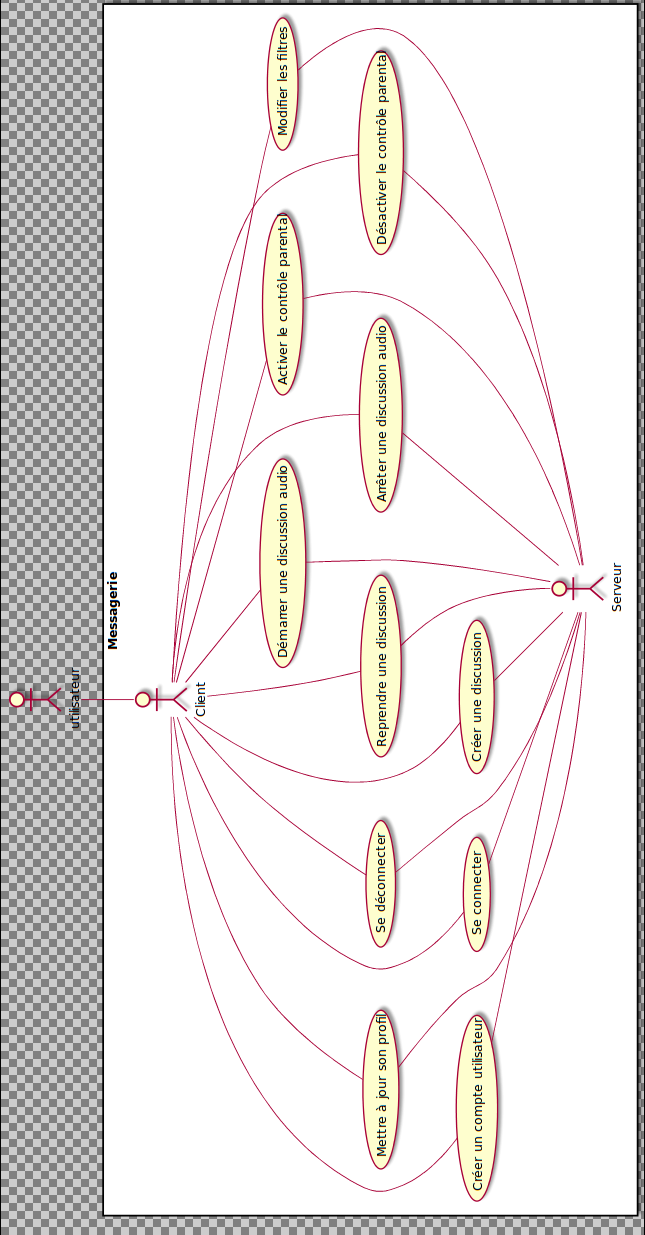
\includegraphics[scale=0.46]{img/usecase.png}
		\caption{Cas d'utilisation}
	\end{figure}
	
	
\subsection{Spécifications d’interface}

\subsubsection{Interface de l’application}

\par L’application devra être responsive design afin d’être consultable autant sur ordinateur, smartphone ou tablette, quelque soit les résolutions d’écrans. 

\par L’interface utilisateur devra être intuitive et facile d’utilisation. 

\subsubsection{Arborescence de l’application web}

\begin{itemize}
	\item Page d'accueil permettant à l’utilisateur de se connecter à la messagerie.	
	\item Une fois connecté page principale de la messagerie contenant les éléments majeurs de l'application web tels que la liste des utilisateurs connectés, l’historique des dernières conversations en ligne et son espace membre avec son image de profil ou avatar.
	\item Page de discussion 
	\item Page de configuration du profil
	\item Page de configuration des filtres
\end{itemize}

\subsubsection{Maquettes}

Écran pour se connecter : 

	\begin{figure}[H]
		\centering 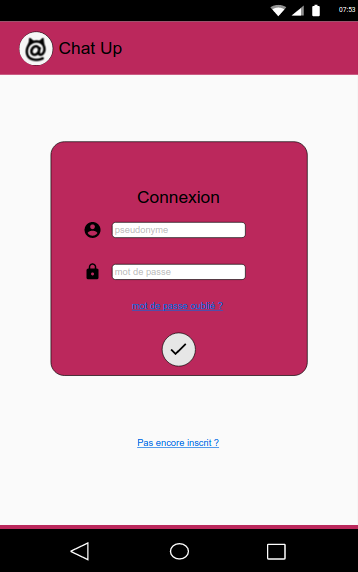
\includegraphics[scale=0.5]{img/SeConnecter.png}
		\caption{Se connecter}
	\end{figure}


Écran de la création de compte :	

	\begin{figure}[H]
		\centering 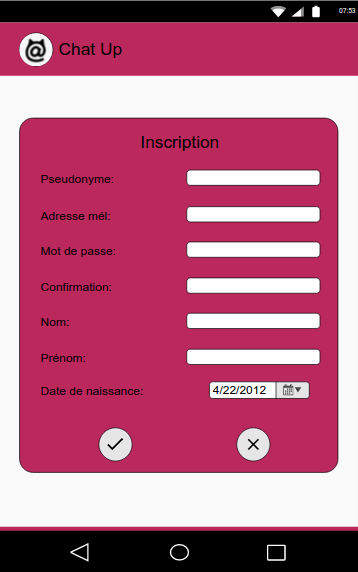
\includegraphics[scale=0.5]{img/CreerUnCompte.png}
		\caption{Créer un compte}
	\end{figure}

	
Écran de la messagerie : 

	\begin{figure}[H]
		\centering 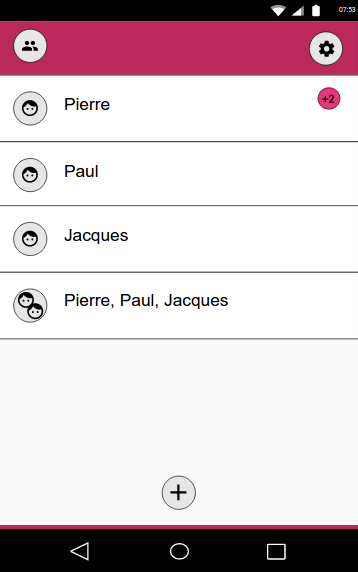
\includegraphics[scale=0.5]{img/Messagerie.png}
		\caption{Messagerie}
	\end{figure}


Écran pour les contacts : 

	\begin{figure}[H]
		\centering 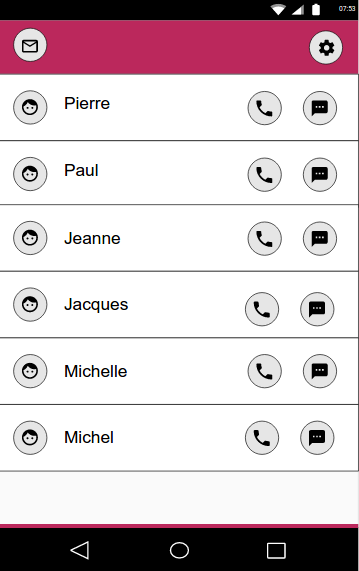
\includegraphics[scale=0.5]{img/Contacts.png}
		\caption{Page des contacts}
	\end{figure}

Écran pour les paramètres : 

	\begin{figure}[H]
		\centering 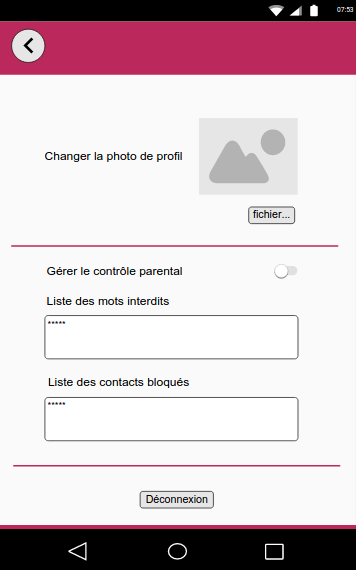
\includegraphics[scale=0.5]{img/Parametres.png}
		\caption{Page de paramètres}
	\end{figure}


Écran d’une conversation textuelle:

	\begin{figure}[H]
		\centering 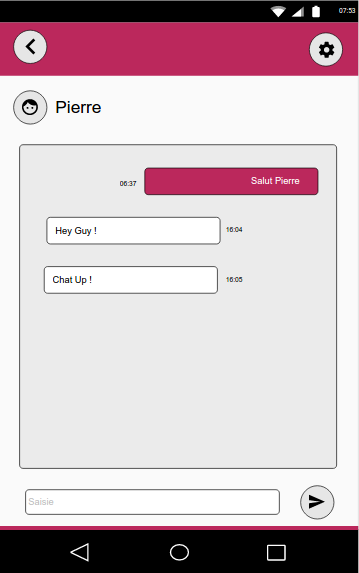
\includegraphics[scale=0.5]{img/Conversation.png}
		\caption{Conversation textuelle}
	\end{figure}

Écran d’une conversation audio :

	\begin{figure}[H]
		\centering 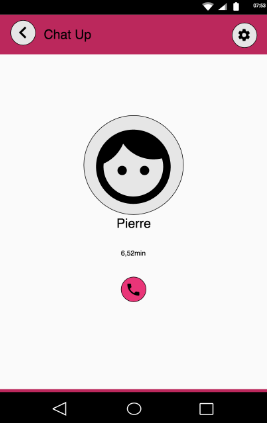
\includegraphics[scale=0.5]{img/audio.png}
		\caption{Conversation audio}
	\end{figure}

\subsubsection{Diagramme de navigation}


	\begin{figure}[H]
		\centering 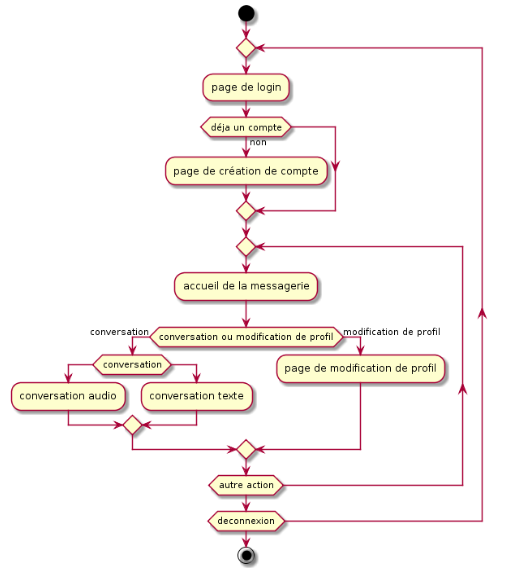
\includegraphics[scale=0.5]{img/diag_navigation.png}
		\caption{Diagramme de navigation}
	\end{figure}
	
	
\subsection{Spécifications opérationnelles}

Performance : La discussion devra être suffisamment rapide pour que la discussion soit instantanée. \\

Sécurité : \\

\begin{itemize}
	\item Les discussions devront être privées et uniquement visibles par les membres de la conversation. 
	\item Les mots de passe des comptes utilisateurs ne seront pas stockés en clair dans la base de données.
\end{itemize}



